\documentclass[18pt]{article}

\usepackage[utf8]{inputenc}
\usepackage[T1]{fontenc}
\usepackage{ragged2e}
\usepackage{caladea}
\usepackage{graphicx}
\usepackage{longtable}
\usepackage{wrapfig}
\usepackage{rotating}
\usepackage{epigraph}
\usepackage[normalem]{ulem}
\usepackage{hyperref}
\usepackage{amsmath}
\usepackage{amssymb}
\usepackage{capt-of}
\usepackage{fancyhdr}

\title{
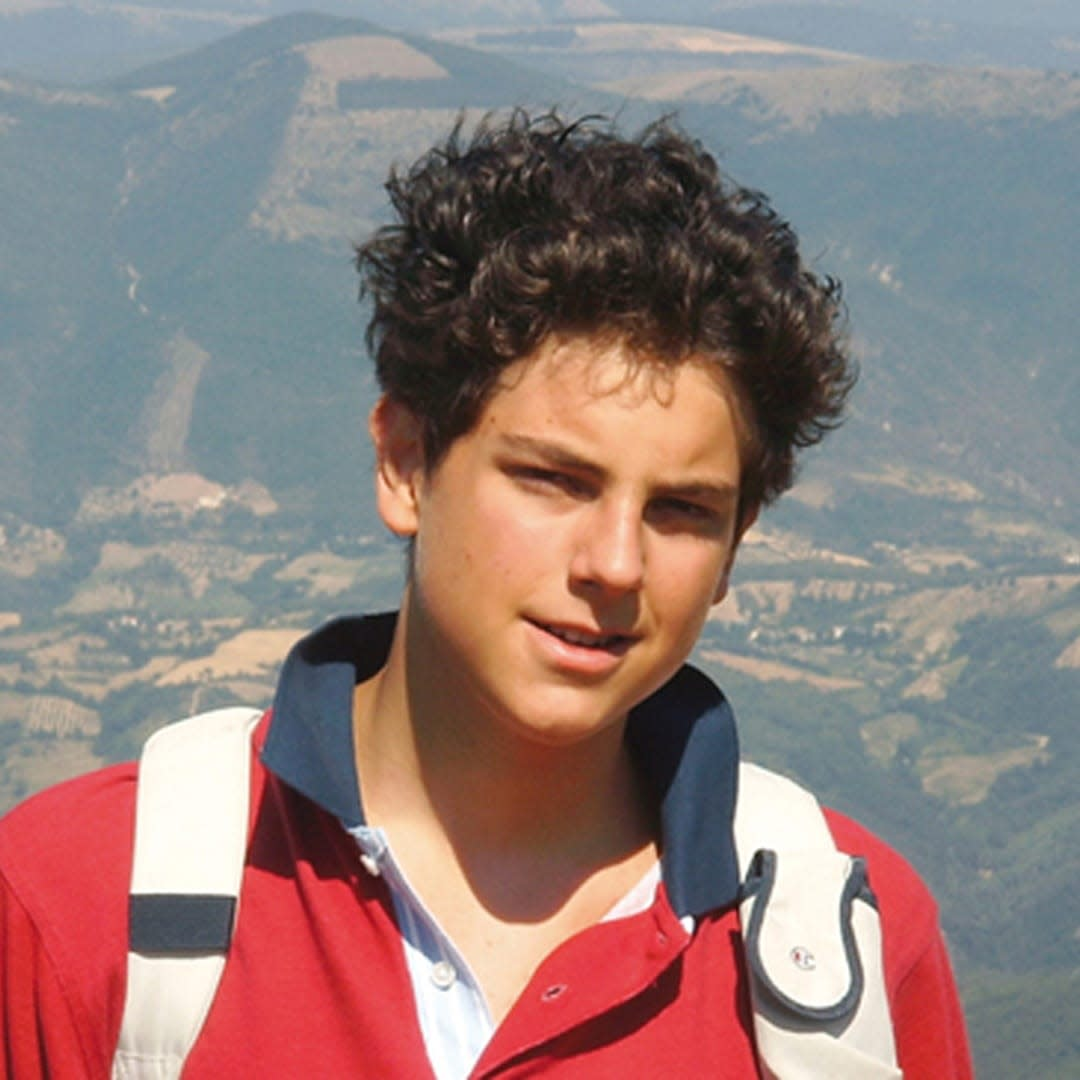
\includegraphics[scale=.54, trim={10cm, 0, 10cm, 0}]{./assets/imagem.jpg}
\par
\vspace{0.5cm}
NOVENA a São Pascoal Baylon
}

\date{Início da Novena : 07/05 \quad Data Litúrgica: 17/05}

\author{Garamog, Nina Freitas}

\renewcommand{\contentsname}{Sumário}

\begin{document}

\maketitle

\tableofcontents

\thispagestyle{empty}

\pagestyle{fancy}
\fancyhf{}
\fancyfoot[LO, CE]{

\includegraphics[scale=0.2]{./assets/cross.png} São Pascoal Baylon, rogai por nós!
}
\fancyfoot[R]{\thepage}

\centering

\vfill

Visite-nos no Telegram: \url{https://t.me/CotidieNovena}

%%%%%%%%%%%%%%%%%%%%%%%%%%%%%%%%%%%% História %%%%%%%%%%%%%%%%%%%%%%%%%%%%%%%%%%%%%%%%%%

\newpage

\begin{justify}
\begin{center}
\section{História}\label{sec:História}
\end{center}

São Pascoal Baylon nasceu em 1540, em Torrehermosa, Aragão, Espanha, em uma família muito pobre e profundamente cristã. Desde criança, trabalhou como pastor de ovelhas, o que favoreceu seu espírito de oração e contemplação. Mesmo analfabeto, Pascoal aprendeu a ler para poder rezar o Ofício da Santíssima Virgem.

Aos 24 anos, ingressou como irmão leigo na Ordem dos Franciscanos Descalços. Destacou-se por sua humildade, penitência, caridade com os pobres e, sobretudo, por seu ardente amor à Eucaristia. Passava longas horas em adoração diante do Santíssimo Sacramento, sendo agraciado com visões e êxtases. Foi também exemplo de pureza, obediência e simplicidade.

São Pascoal faleceu em 17 de maio de 1592, em Villarreal, Espanha. Logo após sua morte, muitos milagres foram atribuídos à sua intercessão, especialmente curas relacionadas à Eucaristia. Foi canonizado em 1690 pelo Papa Alexandre VIII e declarado patrono das obras eucarísticas e dos congressos eucarísticos pelo Papa Leão XIII.

Sua festa é celebrada em 17 de maio. É invocado como protetor dos pobres, dos pastores, dos trabalhadores humildes e, especialmente, dos adoradores do Santíssimo Sacramento.

\vfill

\begin{center}
\href{https://santo.cancaonova.com/santo/sao-pascoal-baylon/}{Fonte: Canção Nova}
\end{center}
\end{justify}

%%%%%%%%%%%%%%%%%%%%%%%%%%%%%%%%%%%%% Orações %%%%%%%%%%%%%%%%%%%%%%%%%%%%%%%%%%%%%%%%%%%

\newpage

\begin{justify}
\begin{center}
\section{Orações}\label{sec:Orações}
\textit{Em nome do Pai, e do Filho, e do Espírito Santo. Amém.}
\end{center}

\subsection*{Ato de Contrição para todos os dias}
Dulcíssimo Jesus meu, em quem creio, em quem espero e a quem amo sobre todas as coisas: por ser Vós suma bondade, me pesa de ter-vos ofendido e proponho, com vossa graça, não voltar a pecar. Amém.

\subsection*{Oração final para todos os dias}
Deus, que ao bem-aventurado São Pascoal, Confessor vosso, honraste com o ardente amor aos sagrados Mistérios de vosso Corpo e Sangue: Concedei-nos propício que, assim como percebeu a espiritual doçura e suavidade deste divino convite, mereçamos também percebê-las nós. Que viveis e reinais pelos séculos dos séculos. Amém.

\vfill
\end{justify}

%%%%%%%%%%%%%%%%%%%%%%%%%%%%%%%%%%%%% Novena - Dias %%%%%%%%%%%%%%%%%%%%%%%%%%%%%%%%%%%%%%%%%%%

\newpage

\section*{Orações de Cada Dia}

\subsection*{Primeiro Dia}
\textbf{Reflexão:}

São Pascoal foi sublimado à excelsitude da santidade, porque foi humildíssimo lego franciscano. Imite-o: embora não sejas humildíssimo, não vos tenhais por virtuoso.

\textbf{Oração:}

Humildíssimo São Pascoal: por amor de Jesus, manso e humilde de coração, vos rogo me outorgueis a virtude da humildade e, com ela, a graça que vos peço nesta novena. Amém.

\textit{Rezar três Pai-Nossos, Ave-Maria e Glória. Terminar com a oração final para todos os dias.}

\subsection*{Segundo Dia}
\textbf{Reflexão:}

São Pascoal foi anjo de inocência, tesouro de angélicas virtudes e, sem dúvida, mortificava duríssimamente seu corpo com asperíssimas penitências. Queres ir ao céu pela senda cômoda dos teus apetites?

\textbf{Oração:}

Santo meu! Alcançai-me do Senhor o espírito de penitência, para que chore minhas culpas passadas e para que não me deixe arrastar jamais por minhas desordenadas paixões. E com esta graça outorgai-me o que vos peço nesta novena. Amém.

\textit{Rezar três Pai-Nossos, Ave-Maria e Glória. Terminar com a oração final para todos os dias.}

\subsection*{Terceiro Dia}
\textbf{Reflexão:}

São Pascoal se fez surdo aos apelos e sorrisos do mundo, desprezando suas promessas e vestindo pobríssimo traje. Não caminhes em busca da vaidade terrena, que o mundo é um mentiroso avaro de seus dons. Imita São Pascoal e aspira aos dons do céu.

\textbf{Oração:}

Amadíssimo São Pascoal: ponde, vos suplico, aversão em minha alma aos prazeres e vaidades loucas do mundo, e um grandíssimo amor às estáveis e puríssimas alegrias da glória, e dai-me a graça que vos peço nesta novena. Amém.

\textit{Rezar três Pai-Nossos, Ave-Maria e Glória. Terminar com a oração final para todos os dias.}

\subsection*{Quarto Dia}
\textbf{Reflexão:}

São Pascoal foi modelo insigne de pureza e inocência de costumes. Menino, pastorzinho, religioso, sempre brilhou nele a graça do candor batismal e o ódio à mais pequena imperfeição. Ama a pureza de vida, que é a felicidade verdadeira.

\textbf{Oração:}

Anjo de pureza, amado São Pascoal: concedei que imite vossa angelical vida, aborrecendo meus pecados, vencendo minhas tentações e vivendo puro na presença do Senhor; e alcançai-me ainda a graça que vos peço nesta novena. Amém.

\textit{Rezar três Pai-Nossos, Ave-Maria e Glória. Terminar com a oração final para todos os dias.}

\subsection*{Quinto Dia}
\textbf{Reflexão:}

São Pascoal viveu na terra sempre unido a Deus, por meio da oração. Seu pensamento, seus desejos, seus suspiros ao céu subiam e no céu estavam. A oração foi para ele tesouro de alegria e mina de santidade. Como vives, apegado sempre à terra sem pensar nunca em vosso Deus, que tanto pensa em ti?

\textbf{Oração:}

Vos suplico, gloriosíssimo São Pascoal, me obtenhais do Senhor o espírito de oração, para que, despegando-me da terra, suspire pela honra que me espera a vosso lado na glória. Concedei também a graça que vos peço nesta novena. Amém.

\textit{Rezar três Pai-Nossos, Ave-Maria e Glória. Terminar com a oração final para todos os dias.}

\subsection*{Sexto Dia}
\textbf{Reflexão:}

São Pascoal amou ardentemente a Deus, como a seu Criador, a seu Redentor, e a seu Pai amantíssimo; e amou terníssimamente as criaturas, como filhas de Deus e como irmãs suas prediletas. Por isto foi amado singularmente de Deus e dos homens. Possuis a virtude excelsa da caridade? O cristão sem caridade é árvore estéril.

\textbf{Oração:}

Por caridade, amadíssimo Santo meu, vos rogo que me deis uma chispa da que inflamava vossa alma, para alentar meu árido coração, e com ela a graça que vos peço nesta novena. Amém.

\textit{Rezar três Pai-Nossos, Ave-Maria e Glória. Terminar com a oração final para todos os dias.}

\subsection*{Sétimo Dia}
\textbf{Reflexão:}

São Pascoal foi serafim extático da Sagrada Eucaristia. Dia e noite velava ante o Sacrário; a Hóstia sacratíssima era o branco de seus desejos e o centro de seus amores. Como agradeces a bondade infinita de Jesus, prisioneiro de amor na terra? Visitá-lo no sacrário e recebê-lo com frequência.

\textbf{Oração:}

Serafim do sacrário, glorioso São Pascoal: fazei que me enamore, como vós, da Sagrada Eucaristia, e que, como vós, sinta fome santíssima de receber a meu Deus sacramentado. Outorgai-me juntamente a graça que vos peço nesta novena. Amém.

\textit{Rezar três Pai-Nossos, Ave-Maria e Glória. Terminar com a oração final para todos os dias.}

\subsection*{Oitavo Dia}
\textbf{Reflexão:}

São Pascoal foi filho amantíssimo da Mãe de Deus e todos os dias a obsequiava com afetuosas mostras de devoção. Amai Maria, pois amá-la é receber suas carícias maternais, é salvar-se.

\textbf{Oração:}

Protetor meu São Pascoal: infundi em meu peito ternura filial à Rainha do Céu, para que me conte entre seus filhos prediletos, na terra e na glória. Concedei também a graça que vos peço nesta novena. Amém.

\textit{Rezar três Pai-Nossos, Ave-Maria e Glória. Terminar com a oração final para todos os dias.}

\subsection*{Nono Dia}
\textbf{Reflexão:}

A morte é o eco da vida. A vida de São Pascoal foi santíssima, e sua morte foi santíssima: um sono dulcíssimo no Senhor. Queres obter boa morte? Imita São Pascoal: vive santamente.

\textbf{Oração:}

Por vossa preciosíssima morte, oh! bendito São Pascoal! vos rogo encarecidamente me consigais do Senhor a graça de não morrer em pecado mortal; a honra de morrer santamente e a felicidade da glória, juntamente com a graça que solicito neste novenário. Amém.

\textit{Rezar três Pai-Nossos, Ave-Maria e Glória. Terminar com a oração final para todos os dias.}

\vfill

\subsection*{Créditos:}
\href{https://www.espacojames.com.br/?cat=54&id=1473}{Espacojames}.

\end{document}
